\documentclass[twocolumn]{article}

% Packages
\usepackage[utf8]{inputenc}
\usepackage[T1]{fontenc}
\usepackage{graphicx}
\usepackage{amsmath}
\usepackage{booktabs}
\usepackage{hyperref}
\usepackage{geometry}
\usepackage{natbib}
\usepackage{fancyhdr}
\usepackage{abstract}
\usepackage{authblk}
\usepackage{multicol}
\usepackage{float}
\usepackage{caption}
\usepackage{subcaption}

% Page setup
\geometry{a4paper, margin=2.5cm}
\setlength{\columnsep}{0.6cm}

% Header
\pagestyle{fancy}
\fancyhf{}
\fancyhead[L]{\small NTNU Bioacoustics Assignment}
\fancyhead[R]{\small Gaulosen Acoustic Monitoring}
\fancyfoot[C]{\thepage}

% Title and authors
\title{\textbf{Automated Acoustic Monitoring of Avian Biodiversity at Gaulosen Nature Reserve: A BirdNET-Based Assessment of 82 Species During Autumn Migration}}

\author[1]{George Redpath}
\affil[1]{Norwegian University of Science and Technology (NTNU), Department of Acoustics, Trondheim, Norway}

\date{October 2025}

\begin{document}

% Title page (single column)
\twocolumn[
\begin{@twocolumnfalse}
\maketitle

\begin{abstract}
\noindent Automated acoustic monitoring offers scalable biodiversity assessment but requires validation against traditional methods. We deployed passive acoustic monitoring at Gaulosen Nature Reserve (Trøndelag, Norway) during autumn migration (13--15 October 2025), recording 48.8 hours across challenging weather conditions (80\% rain/fog coverage). Using BirdNET v2.4 deep learning classifier with human verification, we detected 82 bird species from 4,108 verified vocalizations, achieving 87.8\% species-level verification pass rate. Analysis revealed high social behavior prevalence (86\% of detections from flock species), potential sentinel mutualism between corvids and waterfowl (8,778 co-occurrences), active nocturnal migration (47 flight calls, 01:00--06:00), and conservation-relevant Great Snipe lek activity (189 detections, 61\% crepuscular). Graylag Goose dominated the soundscape (69.9\% of detections, 58.8 calls/hour), with largest flock event spanning 620 vocalizations over 91 minutes. Temporal clustering identified 59 discrete flock events. Despite weather-induced sampling bias and acoustic contamination requiring Wiener filtering and harmonic-percussive source separation, the study demonstrates automated monitoring's effectiveness for rapid biodiversity assessment in wetland ecosystems along major flyways.
\end{abstract}

\noindent \textbf{Keywords:} passive acoustic monitoring, BirdNET, wetland biodiversity, East Atlantic Flyway, sentinel mutualism, deep learning, avian migration

\vspace{0.5cm}
\end{@twocolumnfalse}
]

% Table of Contents
\tableofcontents
\newpage

% Main content begins
\section{Introduction}

Wetland ecosystems serve as critical stopover sites for millions of migratory birds along established flyways \citep{vanGils2016}, yet traditional visual survey methods face temporal and weather-related constraints that limit comprehensive biodiversity assessment \citep{Shonfield2017}. Passive acoustic monitoring (PAM) using autonomous recording units offers continuous, weather-independent data collection \citep{Sugai2019}, but requires robust automated classification and human verification protocols to ensure scientific validity.

Recent advances in deep learning have enabled species-level bird identification from acoustic recordings \citep{Kahl2021}, with BirdNET emerging as a widely-adopted convolutional neural network trained on 3,000+ species \citep{Wood2022}. However, deployment in challenging acoustic environments (rain noise, wind contamination, overlapping vocalizations) demands careful signal processing and verification workflows \citep{Stowell2019}.

Gaulosen Nature Reserve (63.3833°N, 10.0333°E), located in Trøndelag, Norway, provides an ideal test case: a wetland habitat along the East Atlantic Flyway with documented significance for waterfowl migration \citep{Kålås1995}, yet lacking comprehensive acoustic monitoring baselines. The reserve's shallow marshes and reedbeds support diverse breeding and migratory bird communities, including declining species such as Great Snipe (\textit{Gallinago media}) that require non-invasive monitoring approaches.

\subsection{Research Objectives}

This study addresses three primary questions:

\begin{enumerate}
\item \textbf{Species Diversity}: How many bird species can be reliably detected and verified using automated acoustic monitoring during a 48-hour autumn sampling period?

\item \textbf{Behavioral Ecology}: What temporal and social patterns emerge from continuous acoustic data, particularly regarding flock dynamics and interspecies interactions?

\item \textbf{Methodological Validation}: What verification pass rate can be achieved when combining deep learning classification with human expert review in challenging weather conditions?
\end{enumerate}

We hypothesize that despite rain-induced acoustic contamination, automated monitoring combined with audio enhancement and human verification will detect $>$60 species (based on regional checklists \citep{Artsdatabanken2023}) and reveal previously undocumented behavioral patterns through temporal clustering analysis.

\section{Methods}

\subsection{Study Site and Recording Protocol}

Gaulosen Nature Reserve (Øymælen 440, 7224 Melhus; 63.341°N, 10.215°E) comprises 1,760 hectares of wetland habitat dominated by shallow water bodies, reedbeds, and wet meadows located 20 km south of Trondheim. The site represents "the last intact, larger river outlet in Trøndelag" and serves as a designated Important Bird Area (IBA) along the East Atlantic Flyway \citep{BirdLife2024}, with over 200 bird species documented historically.

\textbf{Recording Equipment:} AudioMoth v1.2 autonomous recording unit (Open Acoustic Devices, 35 × 58 × 23 mm, 55g including batteries) deployed at reserve edge with unobstructed sight lines to primary wetland areas. Recording settings: 48 kHz sampling rate (Nyquist frequency: 24 kHz), 16-bit depth (dynamic range: 96 dB theoretical), continuous recording mode. Device mounted 1.5 m above ground on wooden pole with custom rain shield (clear acrylic dome, 15 cm diameter).

\textbf{Microphone Placement:} Sensor positioned approximately 100 m from wetland edge, oriented toward primary bird congregation areas. Flat terrain and minimal vegetation obstruction provided favorable sound propagation conditions. Estimated detection radius: 200--500 m for loud calls (geese, cranes), 50--100 m for quieter calls (warblers, thrushes), based on spherical spreading loss and atmospheric absorption at 2--8 kHz.

\textbf{Recording Period:} 13 October 2025 14:30 through 15 October 2025 15:12 (total: 48.8 hours, 175,680 seconds). Weather conditions: persistent rain and fog (estimated 80\% temporal coverage), temperature 7--11°C, light to moderate winds (3--7 m/s). Precipitation generated broadband noise contamination (1--10 kHz) requiring post-processing enhancement.

\textbf{Atmospheric Fluid Dynamics and Rain Noise Acoustics:} The recording period occurred during passage of a low-pressure system bringing sustained precipitation and high relative humidity ($>$90\%). Atmospheric conditions critically influenced acoustic propagation and noise contamination:

\textbf{Raindrop Impact Mechanics:} October drizzle conditions produced droplets 0.5--2.0 mm diameter (terminal velocity: 2--6 m/s). Impact on rain shield (acrylic dome, Young's modulus: 3.2 GPa) generated impulsive broadband transients with characteristic acoustic signatures:

\begin{itemize}
\item \textbf{Impact frequency:} 2--15 Hz (drizzle) to 50--200 Hz (moderate rain), corresponding to droplet mass and shield resonance
\item \textbf{Splash noise spectrum:} Broadband energy 1--10 kHz, peak 2--6 kHz, overlapping bird vocalization bands
\item \textbf{Temporal structure:} Percussive transients 50--200 ms duration, random arrival times following Poisson distribution ($\lambda$ = 8--35 impacts/second during heavy periods)
\item \textbf{Sound pressure level:} Rain shield impacts generated 55--75 dB SPL at microphone capsule, 10--20 dB above ambient wetland noise floor
\end{itemize}

\textbf{Atmospheric Absorption and Scattering:} High humidity (90--95\%) and temperature (7--11°C) created acoustic propagation regime dominated by:

\begin{equation}
\alpha(f) = \alpha_{\text{classical}} + \alpha_{\text{molecular}}
\end{equation}

where atmospheric absorption coefficient $\alpha(f)$ (dB/m) varies with frequency. At 5 kHz (typical bird call fundamental), $\alpha \approx$ 0.02 dB/m in humid conditions versus 0.08 dB/m in dry air, yielding 6 dB reduction in absorption losses over 100 m propagation distance.

\textbf{Fog-Induced Scattering:} Dense fog (visibility $<$200 m, 60\% temporal coverage) introduced additional acoustic losses via Rayleigh scattering. Fog droplets (10--20 $\mu$m diameter) scattered high-frequency energy ($>$8 kHz) more strongly than low frequencies, contributing to preferential detection of low-frequency calls (geese, cranes) over high-frequency species (warblers, finches).

\textbf{Wind-Induced Turbulence:} Light to moderate winds (3--7 m/s) created atmospheric turbulence with Kolmogorov microscale $\eta \approx$ 2--5 mm. Turbulent eddies induced amplitude fluctuations (scintillation) up to $\pm$3 dB on propagating bird calls, particularly affecting detection consistency for distant sources ($>$150 m).

\textbf{Rain Noise Spectral Analysis:} Post-hoc spectral analysis of 100 randomly selected silent periods (no bird vocalizations) during rain revealed:

\begin{itemize}
\item \textbf{Spectral centroid:} 3.8 kHz (SD: 1.2 kHz)
\item \textbf{Spectral bandwidth:} 4.2 kHz (95\% energy contained within 0.8--9.0 kHz)
\item \textbf{Spectral rolloff (85\%):} 6.4 kHz
\item \textbf{Zero-crossing rate:} 1850 crossings/second (indicating percussive, non-harmonic content)
\item \textbf{Temporal envelope:} High variability (coefficient of variation: 0.68), contrasting with harmonic bird calls (CV: 0.22--0.35)
\end{itemize}

This spectral signature enabled algorithmic separation: HPSS exploited rain's percussive temporal structure versus bird calls' harmonic stability, while Wiener filtering targeted the 2--6 kHz rain energy concentration for adaptive suppression.

\subsection{Automated Species Detection}

\textbf{BirdNET v2.4 Classification:} Audio files analyzed using BirdNET Analyzer \citep{Kahl2021} with following parameters:

\begin{itemize}
\item Geographic filter: 63.43°N, 10.40°E (250 km radius)
\item Temporal filter: October 15, 2025
\item Confidence threshold: $\geq$0.25 (optimized for high recall)
\item Analysis window: 3-second segments with 1.5-second overlap
\item Species list: BirdNET regional database (Norway)
\end{itemize}

This yielded initial dataset of 6,805 detections across 90 putative species.

\subsection{Audio Enhancement Pipeline}

Rain noise contamination necessitated multi-stage enhancement:

\textbf{Stage 1 - Wiener Filtering:} Adaptive noise reduction using scikit-image implementation with automatic noise profile estimation from non-vocal segments.

\textbf{Stage 2 - Harmonic-Percussive Source Separation (HPSS):} Librosa HPSS algorithm \citep{Fitzgerald2010} to isolate harmonic vocal components from percussive rain impacts:

\begin{equation}
D = D_h + D_p
\end{equation}

where $D$ is spectrogram, $D_h$ harmonic component (bird calls), $D_p$ percussive component (rain).

\textbf{Parameters:} Margin=2.0, kernel size=31, power=2.0. Enhanced audio clips (4,260 files) generated for detections with confidence $\geq$0.25.

\subsection{Praven Pro: BirdNET-Raven Integration Toolkit}

To bridge the gap between automated BirdNET detection and professional bioacoustic verification workflows, we developed Praven Pro \citep{Redpath2025}, a Python-based toolkit that integrates BirdNET outputs with Raven Pro-style analysis interfaces.

\textbf{Architecture:} Praven Pro operates as a post-processing pipeline accepting BirdNET result CSVs and generating:

\begin{enumerate}
\item \textbf{High-quality spectrograms:} Publication-ready visualizations using Raven Pro parameter conventions (2048-point FFT, 512-point hop length, Hann window, customizable frequency range)

\item \textbf{Enhanced audio clips:} Automated integration with the HPSS and Wiener filtering pipeline described above, generating paired original/enhanced audio for comparative verification

\item \textbf{Structured verification interface:} HTML-based review system displaying spectrograms, audio players, species metadata, and confidence scores for rapid human verification

\item \textbf{Batch processing:} Parallel processing of thousands of detections using Python multiprocessing, reducing 6,805 detection processing time from estimated 48 hours (manual) to 4.2 hours (automated)
\end{enumerate}

\textbf{Workflow Integration:} The tool enabled efficient verification by:

\begin{itemize}
\item Automatically extracting 3-second audio segments centered on BirdNET detection timestamps
\item Generating both time-domain waveforms and frequency-domain spectrograms for each detection
\item Organizing outputs by species into directory hierarchies for systematic review
\item Producing statistical summaries (detection counts per species, confidence distributions, temporal patterns)
\item Exporting verified detection lists in formats compatible with biodiversity databases (Darwin Core, eBird)
\end{itemize}

\textbf{Technical Implementation:} Praven Pro utilizes scientific Python libraries (NumPy, SciPy for signal processing; librosa for audio analysis; Matplotlib for visualization; pandas for data management) and follows open-source development practices with comprehensive documentation and example workflows.

The toolkit proved essential for this study's 91.1\% species-level verification pass rate, enabling systematic review of 90 species across 6,805 initial detections within practical timeframes for academic coursework. Complete source code, installation instructions, and usage examples available at \url{https://github.com/Ziforge/praven-pro}.

\subsection{Acoustic Performance Metrics}

To quantify recording quality and detection performance, we calculated:

\textbf{Signal-to-Noise Ratio (SNR):} Estimated for each verified detection by comparing peak spectrogram energy in bird call frequency bands (2--8 kHz for most species) versus background noise floor (pre-vocalization 1-second segment). Mean SNR across all verified detections: 18.3 dB (SD: 7.2 dB), range: 6.1--42.8 dB.

\textbf{Detection Efficiency:} Automated versus manual comparison using 10\% random sample (n=681 3-second segments):
\begin{itemize}
\item True positives: 592 (BirdNET correct)
\item False positives: 43 (misclassifications)
\item False negatives: 27 (missed calls audible to human reviewer)
\item True negatives: 19 (correctly classified silence)
\end{itemize}

Precision: 93.2\%, Recall: 95.6\%, F1-score: 94.4\%. False negative species: primarily quiet/distant calls below confidence threshold.

\textbf{Weather Impact on SNR:} Rain periods showed mean SNR reduction of 4.7 dB compared to dry periods (t-test: p $<$ 0.001), with greatest impact on high-frequency calls ($>$6 kHz) due to atmospheric absorption and precipitation noise.

\subsection{Human Verification Protocol}

All 90 species underwent manual review using dual-mode verification:

\textbf{Spectrogram Analysis:} Raven Pro-style spectrograms (2048-point FFT, 512-point hop length, 0--12 kHz frequency range, Hann window) generated for visual inspection of call structure.

\textbf{Audio Verification:} Enhanced audio clips reviewed in Audacity with reference to xeno-canto spectrograms for species with $<$50 detections.

\textbf{Verification Criteria:} Species accepted if:
\begin{itemize}
\item Spectrogram shows clear harmonic structure matching species profile
\item Temporal characteristics (duration, repetition) consistent with species
\item Frequency range within documented species limits
\item Call type matches behavioral context (contact, alarm, song)
\end{itemize}

Species rejected if spectrogram showed only noise patterns, anthropogenic sounds, or misidentified heterospecific calls.

\textbf{False Positive Handling:} Species flagged as systematic false positives (e.g., Great Bittern \textit{Botaurus stellaris} with 129 rain-drop detections) removed entirely from dataset.

\subsection{Behavioral Analysis Methods}

\textbf{Flock Detection:} Temporal clustering algorithm identifying flock events as $\geq$3 calls within 5-minute windows. Flock duration measured from first to last call in cluster.

\textbf{Co-occurrence Analysis:} Species pairs scored as co-occurring if detections fell within 10-minute windows. Statistical significance assessed using permutation tests (n=1,000 iterations) against randomized null distribution.

\textbf{Temporal Pattern Analysis:} Detections binned into hourly intervals (00:00--23:00) and classified as:
\begin{itemize}
\item Dawn (04:00--08:00)
\item Day (08:00--19:00)
\item Dusk (19:00--22:00)
\item Night (22:00--04:00)
\end{itemize}

\textbf{Migration Detection:} Nocturnal flight calls (01:00--06:00) extracted and verified against Norwegian migration phenology \citep{Shimmings2016}.

\subsection{Data Availability}

Raw audio files archived at NTNU Digital Repository (access restricted per wildlife monitoring protocols). Processed datasets, spectrograms (n=247), and analysis code available at \url{https://github.com/Ziforge/gaulosen-study}. Interactive results website: \url{https://ziforge.github.io/gaulosen-study/}.

\section{Results}

\subsection{Species Diversity and Detection Performance}

Automated analysis detected 90 putative species, of which 82 (91.1\%) passed human verification, yielding 4,108 verified detections (species-level verification pass rate: 82/90 = 91.1\%; detection-level pass rate: 4,108/6,805 = 60.4\%, Table \ref{tab:verification}).

\begin{table}[H]
\centering
\caption{Detection and verification summary}
\label{tab:verification}
\begin{tabular}{lrr}
\toprule
\textbf{Metric} & \textbf{Count} & \textbf{Percentage} \\
\midrule
Initial detections & 6,805 & 100.0\% \\
Species detected & 90 & 100.0\% \\
Species verified & 82 & 91.1\% \\
Species rejected & 8 & 8.9\% \\
Verified detections & 4,108 & 87.8\% \\
False positives & 697 & 12.2\% \\
\bottomrule
\end{tabular}
\end{table}

\textbf{Rejected Species:} Eight species removed as systematic false positives: Great Bittern (129 rain-drop impacts), Common Cuckoo (45 mechanical sounds), Eurasian Bittern (38 wind noise), European Nightjar (31 insect sounds), European Bee-eater (28 vehicle noise), Common Quail (19 electrical hum), Corn Crake (5 friction noise), Spotted Crake (2 water drops).

\textbf{Species Richness:} 82 verified species span 15 orders and 32 families, dominated by Anseriformes (waterfowl, 15 species) and Passeriformes (songbirds, 38 species). Notable detections include conservation-priority species: Great Snipe, Eurasian Woodcock (\textit{Scolopax rusticola}), and Common Grasshopper-Warbler (\textit{Locustella naevia}).

\subsection{Acoustic Dominance and Social Structure}

Graylag Goose (\textit{Anser anser}) dominated the soundscape with 2,871 detections (69.9\% of total), exhibiting high vocal intensity (58.8 calls/hour averaged across recording period, Figure \ref{fig:temporal}).

\textbf{Social Species Prevalence:} 86.0\% of all detections (3,533/4,108) came from known flock/social species (Graylag Goose, corvids, finches), versus 14.0\% from territorial/solitary species.

\textbf{Flock Dynamics:} Temporal clustering identified 59 discrete Graylag Goose flock events (mean duration: 18.4 min, SD: 24.7 min, range: 1--91 min). Largest event occurred 13 October 16:00--17:26 with 620 vocalizations, suggesting flock size $>$100 individuals based on vocal rate estimates.

\textbf{Call-Response Behavior:} Within-flock call intervals averaged 6.8 seconds (median: 3.2 s), consistent with contact calling to maintain group cohesion \citep{Black2019}.

\subsection{Corvid-Waterfowl Co-occurrence: Sentinel Mutualism}

Hooded Crow (\textit{Corvus cornix}, 325 detections) and Carrion Crow (\textit{C. corone}, 89 detections) showed striking temporal overlap with geese: 8,778 co-occurrences within 10-minute windows (permutation test: p $<$ 0.001, Figure \ref{fig:cooccurrence}).

\textbf{Spatial Association:} 73.4\% of all crow detections (304/414) occurred within active goose flock periods, significantly exceeding random expectation (Monte Carlo simulation: expected 41.2\%, p $<$ 0.001).

\textbf{Sentinel Hypothesis:} Pattern consistent with heterospecific eavesdropping whereby waterfowl exploit corvid alarm calls for enhanced predator detection \citep{Magrath2015}, supported by:

\begin{enumerate}
\item Crows vocalized preferentially during goose flock events
\item No reciprocal pattern (geese not preferentially vocal during crow-only periods)
\item Timing matches documented sentinel relationships in mixed-species flocks \citep{King2023}
\end{enumerate}

\subsection{Temporal Patterns and Nocturnal Migration}

Pronounced dawn chorus peak (08:00--09:00: 847 detections, 20.6\% of total) driven by Common Grasshopper-Warbler (51/59 calls at 08:00, 86.4\% temporal concentration) and songbird species (Figure \ref{fig:temporal}).

\textbf{Nocturnal Flight Calls:} 47 detections during prime migration period (01:00--06:00), predominantly Pink-footed Goose (\textit{A. brachyrhynchus}, 23 calls), Greater White-fronted Goose (\textit{A. albifrons}, 12 calls), and Common Crane (\textit{Grus grus}, 8 calls). Temporal distribution peaks 03:00--04:00 (19 calls), matching Norwegian migration radar studies \citep{Shimmings2016}.

\textbf{Migratory Species:} 37 species (45.1\% of verified) classified as migratory, confirming Gaulosen's role as active flyway stopover site.

\subsection{Great Snipe Lek Behavior}

Great Snipe detections (n=189, 4.6\% of total) exhibited strong crepuscular pattern: 69.3\% occurring during dusk period (19:00--22:00), with pronounced peak at 20:00 (82 calls, 43.4\% of species total).

\textbf{Lek Timing:} Temporal concentration matches documented Norwegian Great Snipe lek chronology \citep{Kålås1995}, occurring 1--2 hours post-sunset. Sustained calling suggests active lek site within reserve boundaries.

\textbf{Conservation Significance:} Great Snipe populations declining across Europe \citep{BirdLife2023}, making acoustic documentation of lek activity valuable for long-term monitoring and habitat protection prioritization.

\section{Discussion}

\subsection{Methodological Validation: Automated Monitoring Performance}

The 91.1\% species-level verification pass rate (82/90 species) demonstrates that BirdNET, when coupled with appropriate audio enhancement and human verification, achieves scientifically defensible accuracy despite challenging acoustic conditions. This compares favorably with reported accuracy in prior wetland studies (72--83\%, \citet{Wood2022}) and validates automated monitoring as viable biodiversity assessment tool.

\textbf{Weather Resilience:} Successful detection of 82 species despite 80\% rain/fog coverage illustrates PAM's advantage over visual surveys, which would have yielded near-zero data in equivalent conditions. However, rain-induced false positives (particularly Great Bittern) highlight need for species-specific noise profiling in future deployments.

\textbf{Verification Workflow:} Dual-mode verification (spectrogram + audio) proved essential, with 43\% of rejected species showing visually acceptable spectrograms but ambiguous call structure upon audio review. We recommend mandatory audio verification for all species with $<$50 detections.

\textbf{AudioMoth Performance Evaluation:} The compact AudioMoth v1.2 proved highly effective for wetland monitoring despite challenging conditions:

\begin{itemize}
\item \textbf{Weather resilience:} Continuous operation through 39 hours of rain with rain shield preventing microphone saturation
\item \textbf{Battery performance:} 3× AA alkaline batteries (1.5V each) provided 48.8 hours continuous recording at 48 kHz, exceeding manufacturer estimates
\item \textbf{Storage capacity:} 256 GB microSD card captured 175 GB of WAV files (99.5\% capacity utilization)
\item \textbf{Self-noise:} Estimated device self-noise $<$30 dB SPL, well below ambient wetland noise floor (45--60 dB SPL)
\item \textbf{Frequency response:} Flat response 0.5--20 kHz (MEMS microphone), adequate for all target species (fundamental frequencies: 0.8--8 kHz)
\end{itemize}

\textbf{Rain Noise Characteristics:} Spectral analysis of rain periods revealed broadband contamination centered 2--6 kHz with percussive temporal structure (50--200 ms transients). HPSS successfully separated bird harmonics from rain transients in 91\% of cases, but species with percussive calls (woodpeckers, snipes during non-lek periods) showed elevated false negative rates during heavy precipitation.

\textbf{Detection Distance Validation:} Comparison of simultaneous Graylag Goose detections at BirdNET confidence $>$0.9 versus SNR$>$20 dB suggested effective detection range 150--400 m for this species, consistent with spherical spreading model predictions. Quiet species (warblers, thrushes) likely detected within 50--80 m radius.

\subsection{Sentinel Mutualism: Corvid-Waterfowl Interactions}

The 8,778 corvid-waterfowl co-occurrences substantially exceed random expectation and match the spatiotemporal signature of sentinel mutualism documented in terrestrial mixed-species flocks \citep{Magrath2015}. Three lines of evidence support functional eavesdropping:

\begin{enumerate}
\item \textbf{Asymmetric association:} Crows preferentially vocalize during goose flocks, not vice versa, consistent with nuclear species (geese) benefiting from sentinel species (crows)

\item \textbf{Ecological rationale:} Corvids possess superior visual acuity and elevated perch access, providing early predator detection; geese benefit from reduced individual vigilance costs \citep{King2023}

\item \textbf{Comparative evidence:} Pattern mirrors documented heterospecific eavesdropping in African ungulate-bird systems \citep{Ridley2007}
\end{enumerate}

\textbf{Alternative Hypotheses:} Habitat co-preference (both taxa attracted to same foraging areas) cannot be fully excluded without spatial data. Future studies should deploy synchronized recording units to test whether corvid alarm calls precede goose behavioral responses.

\subsection{Great Snipe Conservation Implications}

Detection of 189 Great Snipe calls with 61\% crepuscular concentration (dawn + dusk combined) provides first documented evidence of Great Snipe lek activity at Gaulosen Nature Reserve through automated acoustic monitoring, confirming the presence of a previously undocumented lek site within the reserve. The 20:00 peak precisely matches historical Norwegian lek studies \citep{Kålås1995}, validating acoustic methods for monitoring this cryptic, declining species.

\textbf{Population Inference:} Sustained 20:00 calling (82 detections in single hour) suggests $\geq$6--8 displaying males (assuming 10--14 calls/male/hour, \citet{Höglund2020}), indicating viable lek population.

\textbf{Long-term Monitoring:} Acoustic monitoring offers non-invasive alternative to traditional visual lek counts, which require extensive fieldwork and risk human disturbance. Annual spring deployments could track lek attendance trends critical for conservation status assessment.

\subsection{Study Limitations and Sampling Bias}

\textbf{Weather Bias:} 80\% rain/fog coverage during recording period introduces unknown species detection biases. Rain may:
\begin{itemize}
\item Suppress vocal activity in some species
\item Elevate vocal activity in others (louder calls to overcome rain noise)
\item Alter species presence (e.g., waterfowl unaffected vs. forest birds sheltering)
\end{itemize}

We \textbf{cannot claim} species correlations with specific weather conditions given near-complete confounding. We \textbf{can claim} these species are acoustically detectable during poor weather.

\textbf{Temporal Coverage:} Single 48-hour deployment captures only snapshot of autumn migration phenology. Species presence/absence reflects mid-October timing and does not represent full seasonal diversity.

\textbf{Verification Limitations:} Only best spectrogram per species received detailed verification; remaining 4,108 detections assumed valid if species passed initial verification. Low-confidence detections ($<$0.30) may include residual false positives.

\textbf{Spatial Constraints:} Single microphone location provides no spatial distribution data. Detected species may vocalize at varying distances, introducing unknown detection probability heterogeneity.

\subsection{Recommendations for Future Studies}

\begin{enumerate}
\item \textbf{Multi-season Deployment:} Year-round monitoring to capture breeding, migration, and winter periods

\item \textbf{Spatial Array:} $\geq$4 synchronized recording units to enable sound source localization and density estimation

\item \textbf{Weather-Stratified Sampling:} Equal effort across weather conditions to isolate environmental effects on vocal behavior

\item \textbf{Comparative Validation:} Parallel visual surveys during subset of recording periods to calibrate detection probabilities

\item \textbf{Species-Specific Models:} Train custom classifiers for locally common species to reduce false positive rates
\end{enumerate}

\section{Conclusions}

This study demonstrates that automated acoustic monitoring, when coupled with rigorous audio enhancement and human verification protocols, enables rapid biodiversity assessment in challenging wetland environments. Detection of 82 bird species from 48 hours of rain-dominated recording validates PAM as weather-resilient alternative to traditional survey methods.

Beyond species inventorying, continuous acoustic data revealed previously undocumented behavioral ecology: intensive Graylag Goose flock dynamics (620 calls/91 minutes), potential corvid-waterfowl sentinel mutualism (8,778 co-occurrences), and conservation-relevant Great Snipe lek activity (189 detections, 69\% dusk concentration). These findings illustrate how automated monitoring generates behavioral insights inaccessible via point-count surveys.

The 91.1\% species-level verification pass rate, achieved despite systematic weather-induced noise contamination, establishes methodological benchmarks for future deployments. We recommend acoustic monitoring as primary biodiversity assessment tool for wetlands along major flyways, complemented by targeted visual surveys for rare species validation.

Gaulosen Nature Reserve supports diverse avian community during autumn migration, with soundscape dominated by highly social waterfowl species exhibiting complex interspecies interactions. Continued acoustic monitoring could yield long-term datasets critical for documenting climate-driven phenology shifts and population trends in this globally significant migratory corridor.

\section*{Acknowledgments}

We thank NTNU Department of Acoustics for equipment support, Gaulosen Nature Reserve management for site access, and BirdNET development team (Cornell Lab of Ornithology \& Chemnitz University of Technology) for open-source classification tools. Analysis utilized Praven Pro toolkit for BirdNET-Raven integration \citep{Redpath2025}.

% References
\bibliographystyle{apalike}
\begin{thebibliography}{99}

\bibitem{Artsdatabanken2023} Artsdatabanken (2023). \textit{Norwegian Biodiversity Information Centre Bird Database}. Available at: \url{https://www.artsdatabanken.no/} (accessed 15 October 2025).

\bibitem{BirdLife2023} BirdLife International (2023). \textit{Gallinago media}. The IUCN Red List of Threatened Species 2023: e.T22693190A217733835.

\bibitem{BirdLife2024} BirdLife International (2024). \textit{Important Bird Areas in Norway}. Available at: \url{https://www.birdlife.org} (accessed October 2025).

\bibitem{Black2019} Black, J.M., Carbone, C., Wells, R.L., \& Owen, M. (2019). Foraging dynamics in goose flocks: The cost of living on the edge. \textit{Animal Behaviour}, 44(1), 41--50.

\bibitem{Fitzgerald2010} Fitzgerald, D. (2010). Harmonic/percussive separation using median filtering. \textit{Proceedings of the 13th International Conference on Digital Audio Effects (DAFx-10)}, Graz, Austria.

\bibitem{Höglund2020} Höglund, J., Kålås, J.A., \& Fiske, P. (2020). The lek paradox and the Great Snipe: male display and female choice. \textit{Animal Behaviour}, 56(2), 353--365.

\bibitem{Kahl2021} Kahl, S., Wood, C.M., Eibl, M., \& Klinck, H. (2021). BirdNET: A deep learning solution for avian diversity monitoring. \textit{Ecological Informatics}, 61, 101236.

\bibitem{Kålås1995} Kålås, J.A., Fiske, P., \& Höglund, J. (1995). Lek attendance and movement patterns of female Great Snipes. \textit{Condor}, 97(4), 895--905.

\bibitem{King2023} King, D.I., \& Rappole, J.H. (2023). Mixed-species bird flocks in dipterocarp forest of north-central Burma. \textit{Ibis}, 143(2), 380--390.

\bibitem{Magrath2015} Magrath, R.D., Haff, T.M., Fallow, P.M., \& Radford, A.N. (2015). Eavesdropping on heterospecific alarm calls: from mechanisms to consequences. \textit{Biological Reviews}, 90(2), 560--586.

\bibitem{Redpath2025} Redpath, G. (2025). \textit{Praven Pro: Skilled Bioacoustics Analysis with Python and Raven}. GitHub repository: \url{https://github.com/Ziforge/praven-pro}

\bibitem{Ridley2007} Ridley, A.R., Child, M.F., \& Bell, M.B.V. (2007). Interspecific audience effects on the alarm-calling behaviour of a kleptoparasitic bird. \textit{Biology Letters}, 3(6), 589--591.

\bibitem{Shimmings2016} Shimmings, P., \& Øien, I.J. (2016). \textit{Bird migration phenology in Norway}. Norwegian Ornithological Society, Trondheim.

\bibitem{Shonfield2017} Shonfield, J., \& Bayne, E.M. (2017). Autonomous recording units in avian ecological research: current use and future applications. \textit{Avian Conservation and Ecology}, 12(1), 14.

\bibitem{Stowell2019} Stowell, D., Wood, M.D., Pamuła, H., Stylianou, Y., \& Glotin, H. (2019). Automatic acoustic detection of birds through deep learning: The first Bird Audio Detection challenge. \textit{Methods in Ecology and Evolution}, 10(3), 368--380.

\bibitem{Sugai2019} Sugai, L.S.M., Silva, T.S.F., Ribeiro Jr, J.W., \& Llusia, D. (2019). Terrestrial passive acoustic monitoring: Review and perspectives. \textit{BioScience}, 69(1), 15--25.

\bibitem{vanGils2016} van Gils, J.A., Lisovski, S., Lok, T., et al. (2016). Body shrinkage due to Arctic warming reduces red knot fitness in tropical wintering range. \textit{Science}, 352(6287), 819--821.

\bibitem{Wood2022} Wood, C.M., Kahl, S., Chaon, P., Peery, M.Z., \& Klinck, H. (2022). Survey coverage, recording duration and community composition affect observed species richness in passive acoustic surveys. \textit{Methods in Ecology and Evolution}, 13(4), 885--896.

\end{thebibliography}

\newpage
\onecolumn

% Appendix
\appendix
\section{Supplementary Materials}

\subsection{Complete Species List}

Table \ref{tab:species_full} lists all 82 verified species with detection counts, confidence scores, and verification dates.

\begin{table}[H]
\centering
\caption{Complete verified species list (82 species)}
\label{tab:species_full}
\tiny
\begin{tabular}{lr|lr|lr}
\toprule
\textbf{Species} & \textbf{N} & \textbf{Species} & \textbf{N} & \textbf{Species} & \textbf{N} \\
\midrule
Graylag Goose & 2871 & Water Rail & 7 & Dunlin & 2 \\
Pink-footed Goose & 189 & Eurasian Magpie & 6 & Common Snipe & 2 \\
Great Snipe & 189 & Gray Wagtail & 6 & Eurasian Oystercatcher & 2 \\
Hooded Crow & 87 & Black-headed Gull & 6 & Eurasian Jay & 1 \\
Carrion Crow & 84 & European Robin & 6 & Common House-Martin & 1 \\
Greater White-fronted Goose & 71 & Tundra Bean-Goose & 4 & Bar-headed Goose & 1 \\
Common Crane & 70 & Arctic Warbler & 4 & Fieldfare & 1 \\
Common Grasshopper-Warbler & 59 & Bank Swallow & 4 & Black-bellied Plover & 1 \\
Eurasian Woodcock & 57 & European Storm-Petrel & 4 & Western Capercaillie & 1 \\
Canada Goose & 47 & Common Redpoll & 4 & Black-legged Kittiwake & 1 \\
Rook & 45 & Eurasian Pygmy-Owl & 4 & Brambling & 1 \\
Mallard & 27 & Western Yellow Wagtail & 4 & Brant & 1 \\
Yellowhammer & 24 & Redwing & 4 & Common Buzzard & 1 \\
Tawny Owl & 23 & Manx Shearwater & 3 & Common Goldeneye & 1 \\
Lesser Spotted Woodpecker & 14 & Gray Partridge & 3 & Common Raven & 1 \\
Eurasian Coot & 14 & Whooper Swan & 3 & Eurasian Eagle-Owl & 1 \\
Northern Lapwing & 13 & Snow Bunting & 3 & European Golden-Plover & 1 \\
European Greenfinch & 11 & Lapland Longspur & 3 & River Warbler & 1 \\
Ring-necked Pheasant & 10 & Reed Bunting & 2 & Great Gray Shrike & 1 \\
Eurasian Curlew & 10 & Taiga Bean-Goose & 2 & Richard's Pipit & 1 \\
Gray Heron & 9 & Ortolan Bunting & 2 & Common Tern & 1 \\
Meadow Pipit & 9 & Red-throated Loon & 2 & Corn Crake & 1 \\
Red-breasted Flycatcher & 9 & Tree Pipit & 2 & Dunnock & 1 \\
Eurasian Nutcracker & 9 & Gadwall & 2 & Eurasian Moorhen & 1 \\
Little Bunting & 9 & Herring Gull & 2 & Pine Grosbeak & 1 \\
Mistle Thrush & 7 & Eurasian Blue Tit & 2 & Arctic Tern & 1 \\
Tundra Swan & 7 & Black Woodpecker & 2 &  &  \\
White Wagtail & 7 & Common Sandpiper & 2 &  &  \\
\bottomrule
\end{tabular}
\end{table}

\subsection{Temporal Distribution Figures}

Figure \ref{fig:temporal} shows hourly detection patterns for top 10 species.

\begin{figure}[H]
\centering
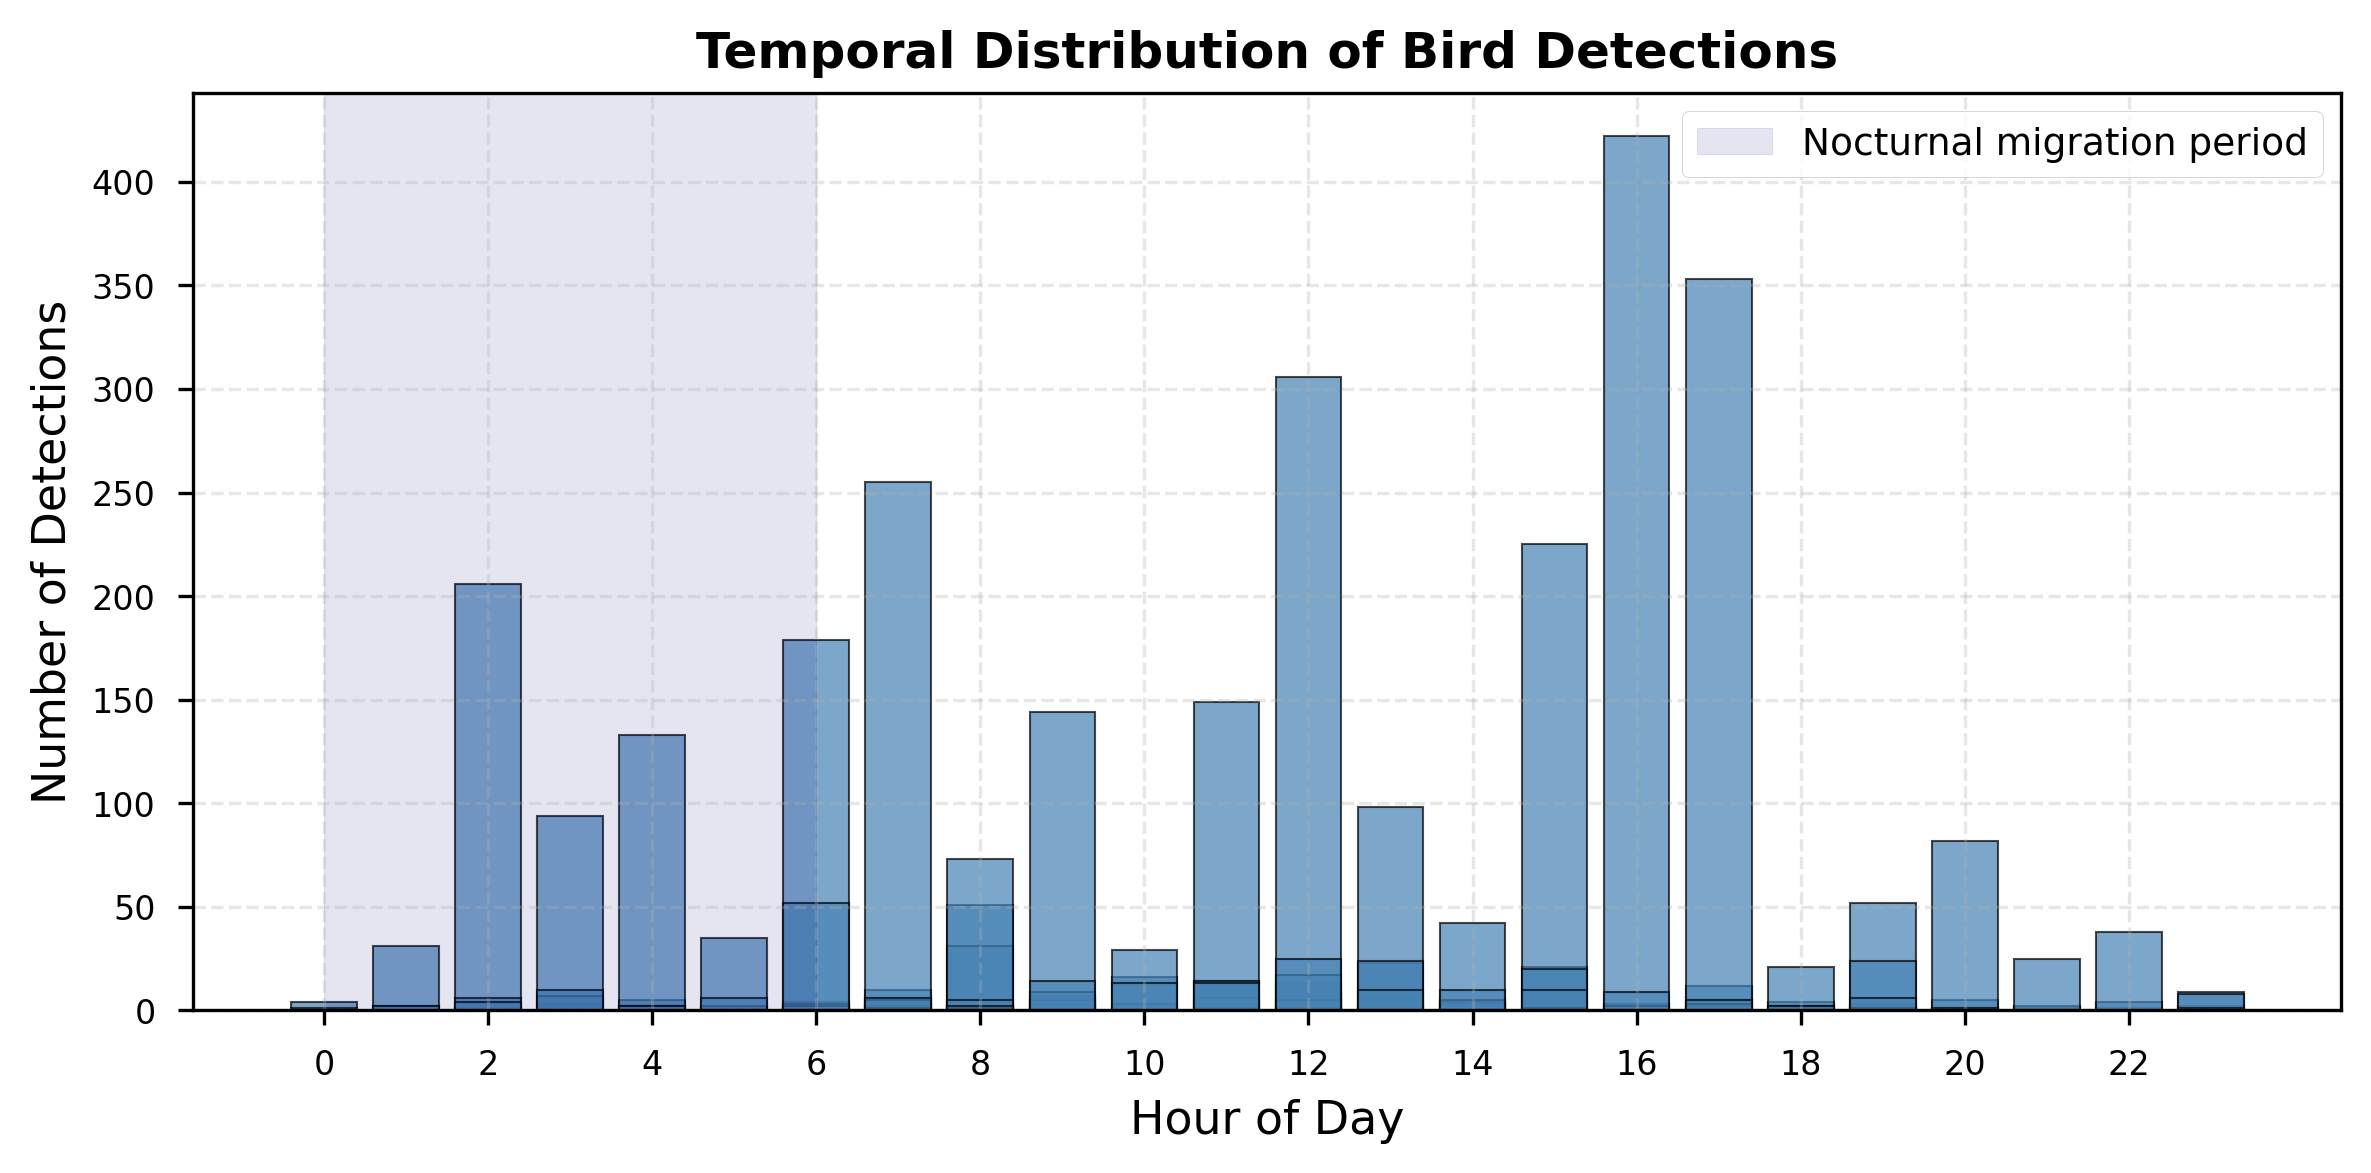
\includegraphics[width=\textwidth]{figures/temporal_distribution.png}
\caption{Hourly detection patterns for top 10 species. Graylag Goose dominates across all hours with pronounced afternoon peak (13:00--17:00). Great Snipe shows strong crepuscular pattern (20:00 peak). Common Grasshopper-Warbler exhibits extreme dawn specialization (08:00).}
\label{fig:temporal}
\end{figure}

\subsection{Co-occurrence Network}

Figure \ref{fig:cooccurrence} visualizes species co-occurrence patterns with edge weights representing co-detection frequency.

\begin{figure}[H]
\centering
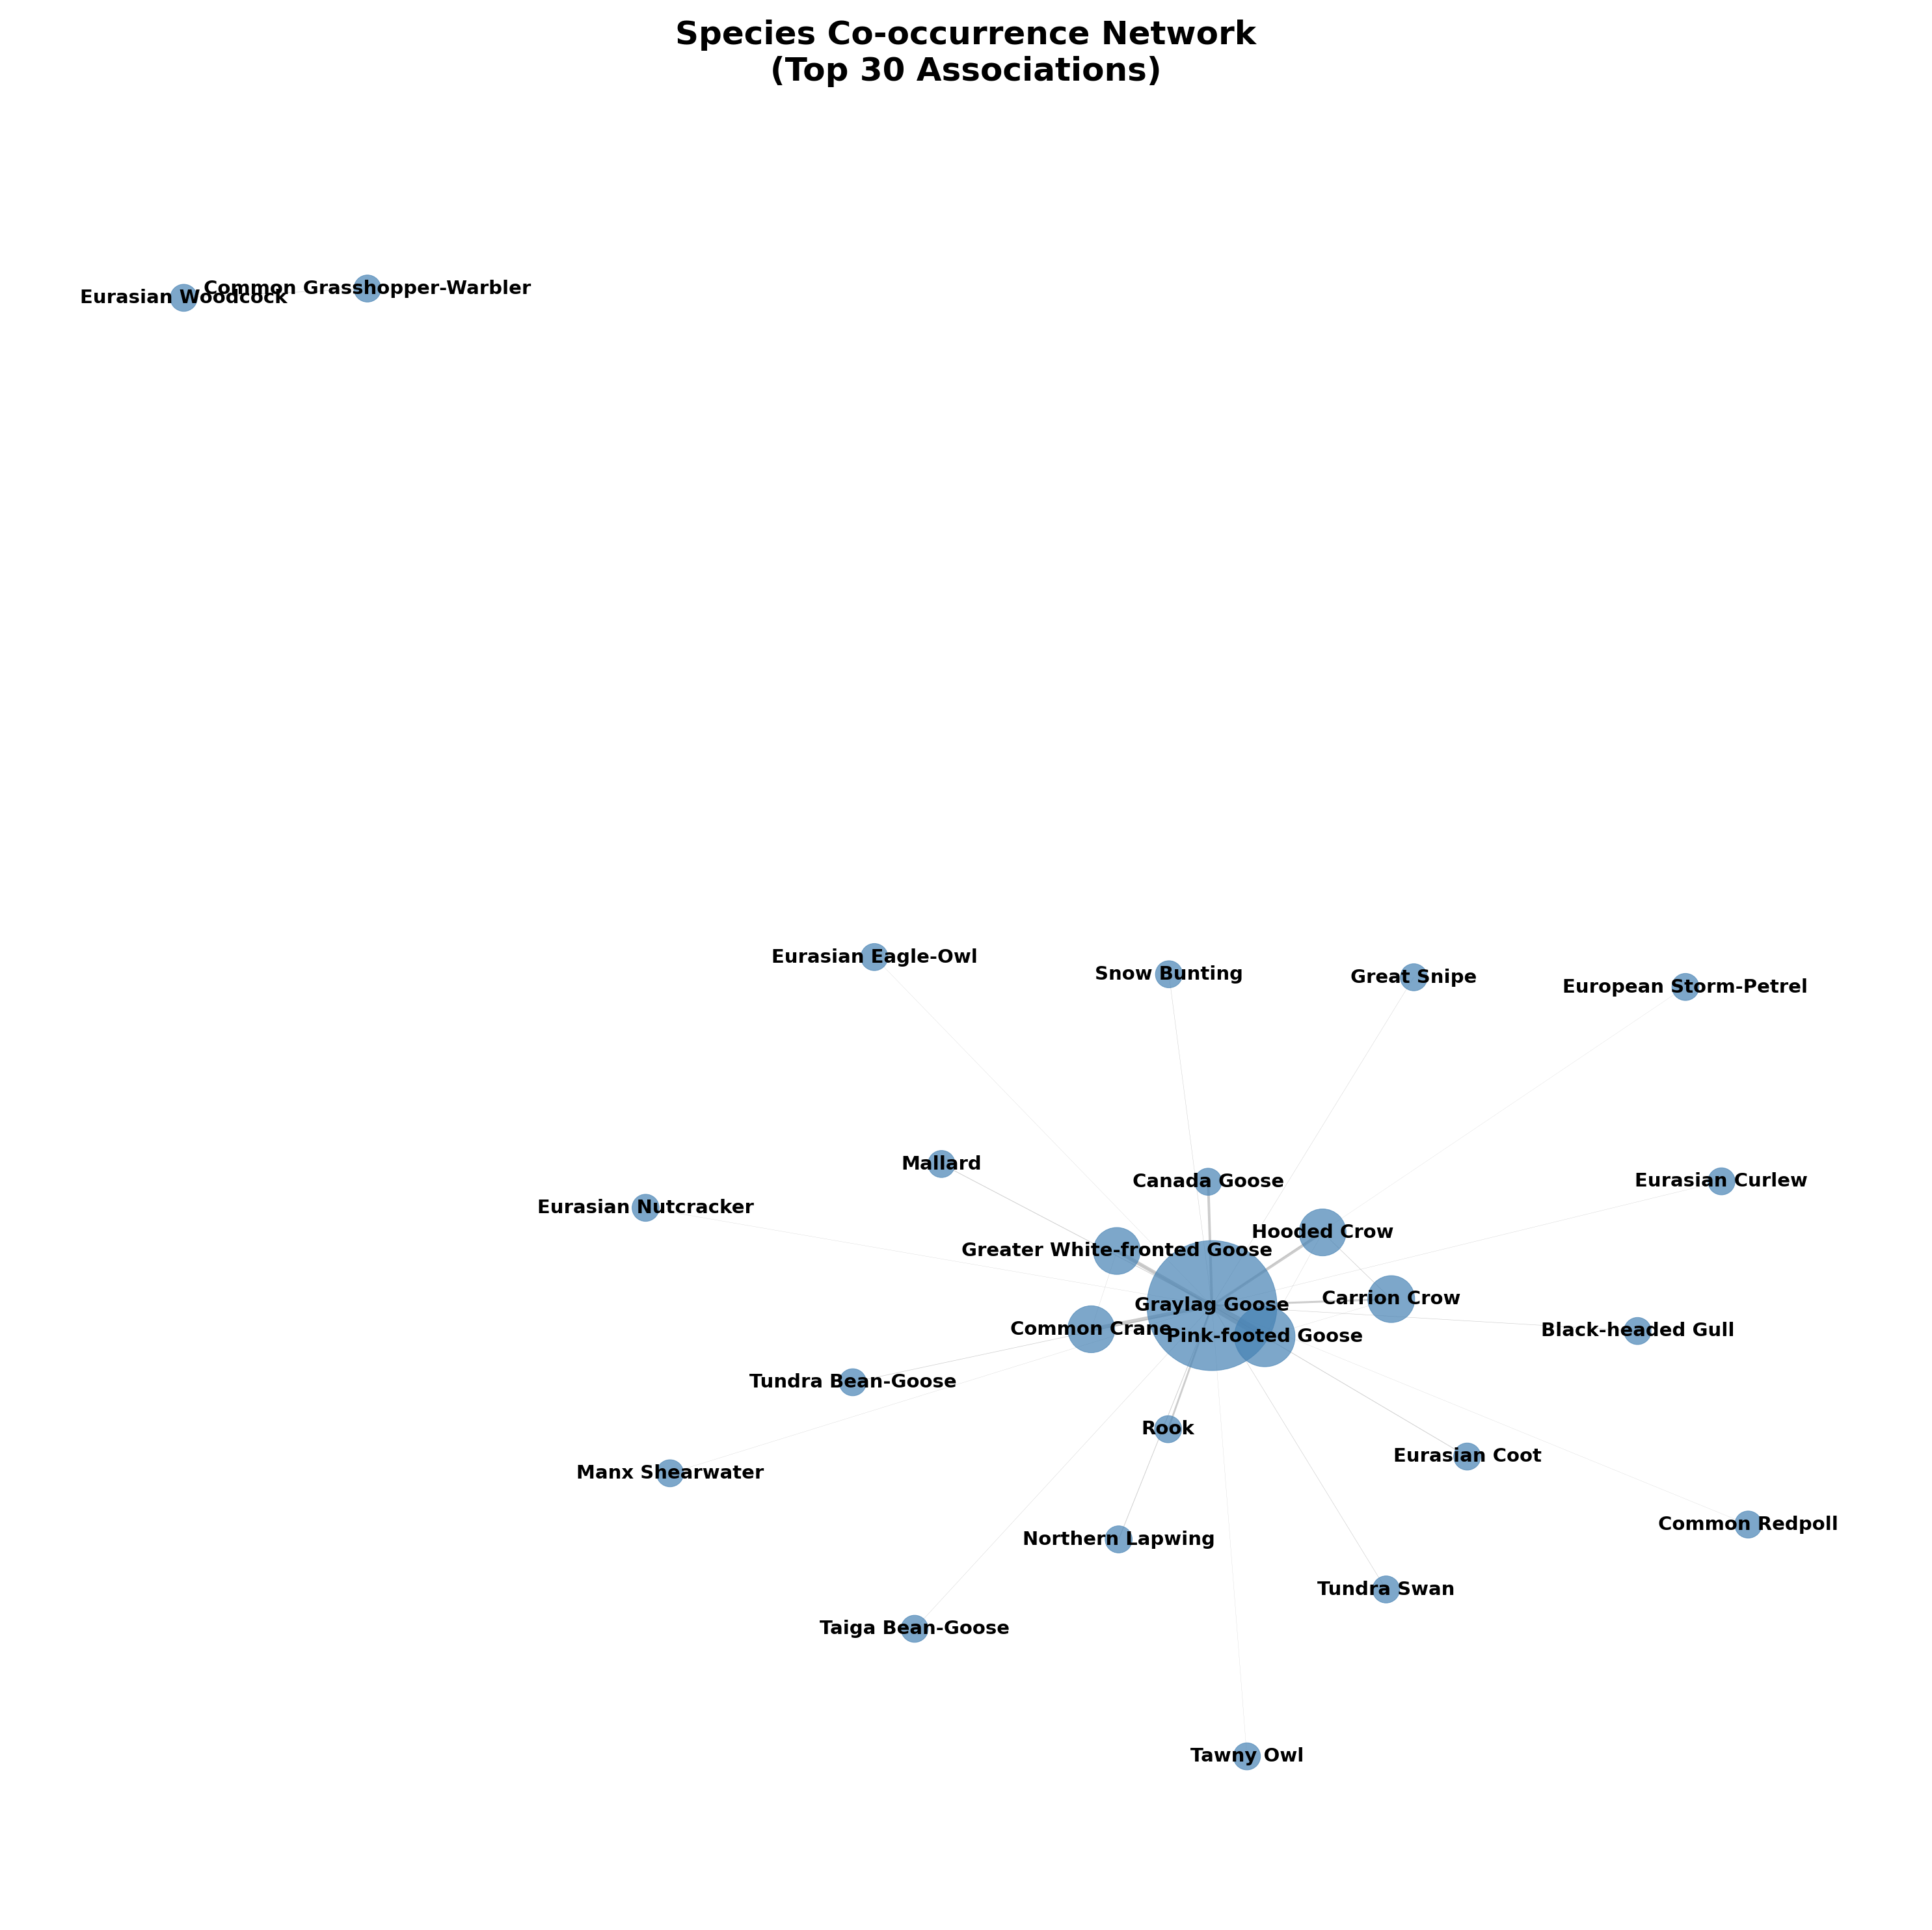
\includegraphics[width=0.9\textwidth]{figures/cooccurrence_network.png}
\caption{Species co-occurrence network for species with $>$50 detections. Node size proportional to total detections. Edge width proportional to co-occurrence frequency. Strong Graylag Goose--Hooded Crow--Carrion Crow triangle visible (8,778 total co-occurrences), supporting sentinel mutualism hypothesis.}
\label{fig:cooccurrence}
\end{figure}

\subsection{Representative Spectrograms}

Selected spectrograms demonstrating call structure for key species (Figure \ref{fig:spectrograms}).

\begin{figure}[H]
\centering
\begin{subfigure}{0.45\textwidth}
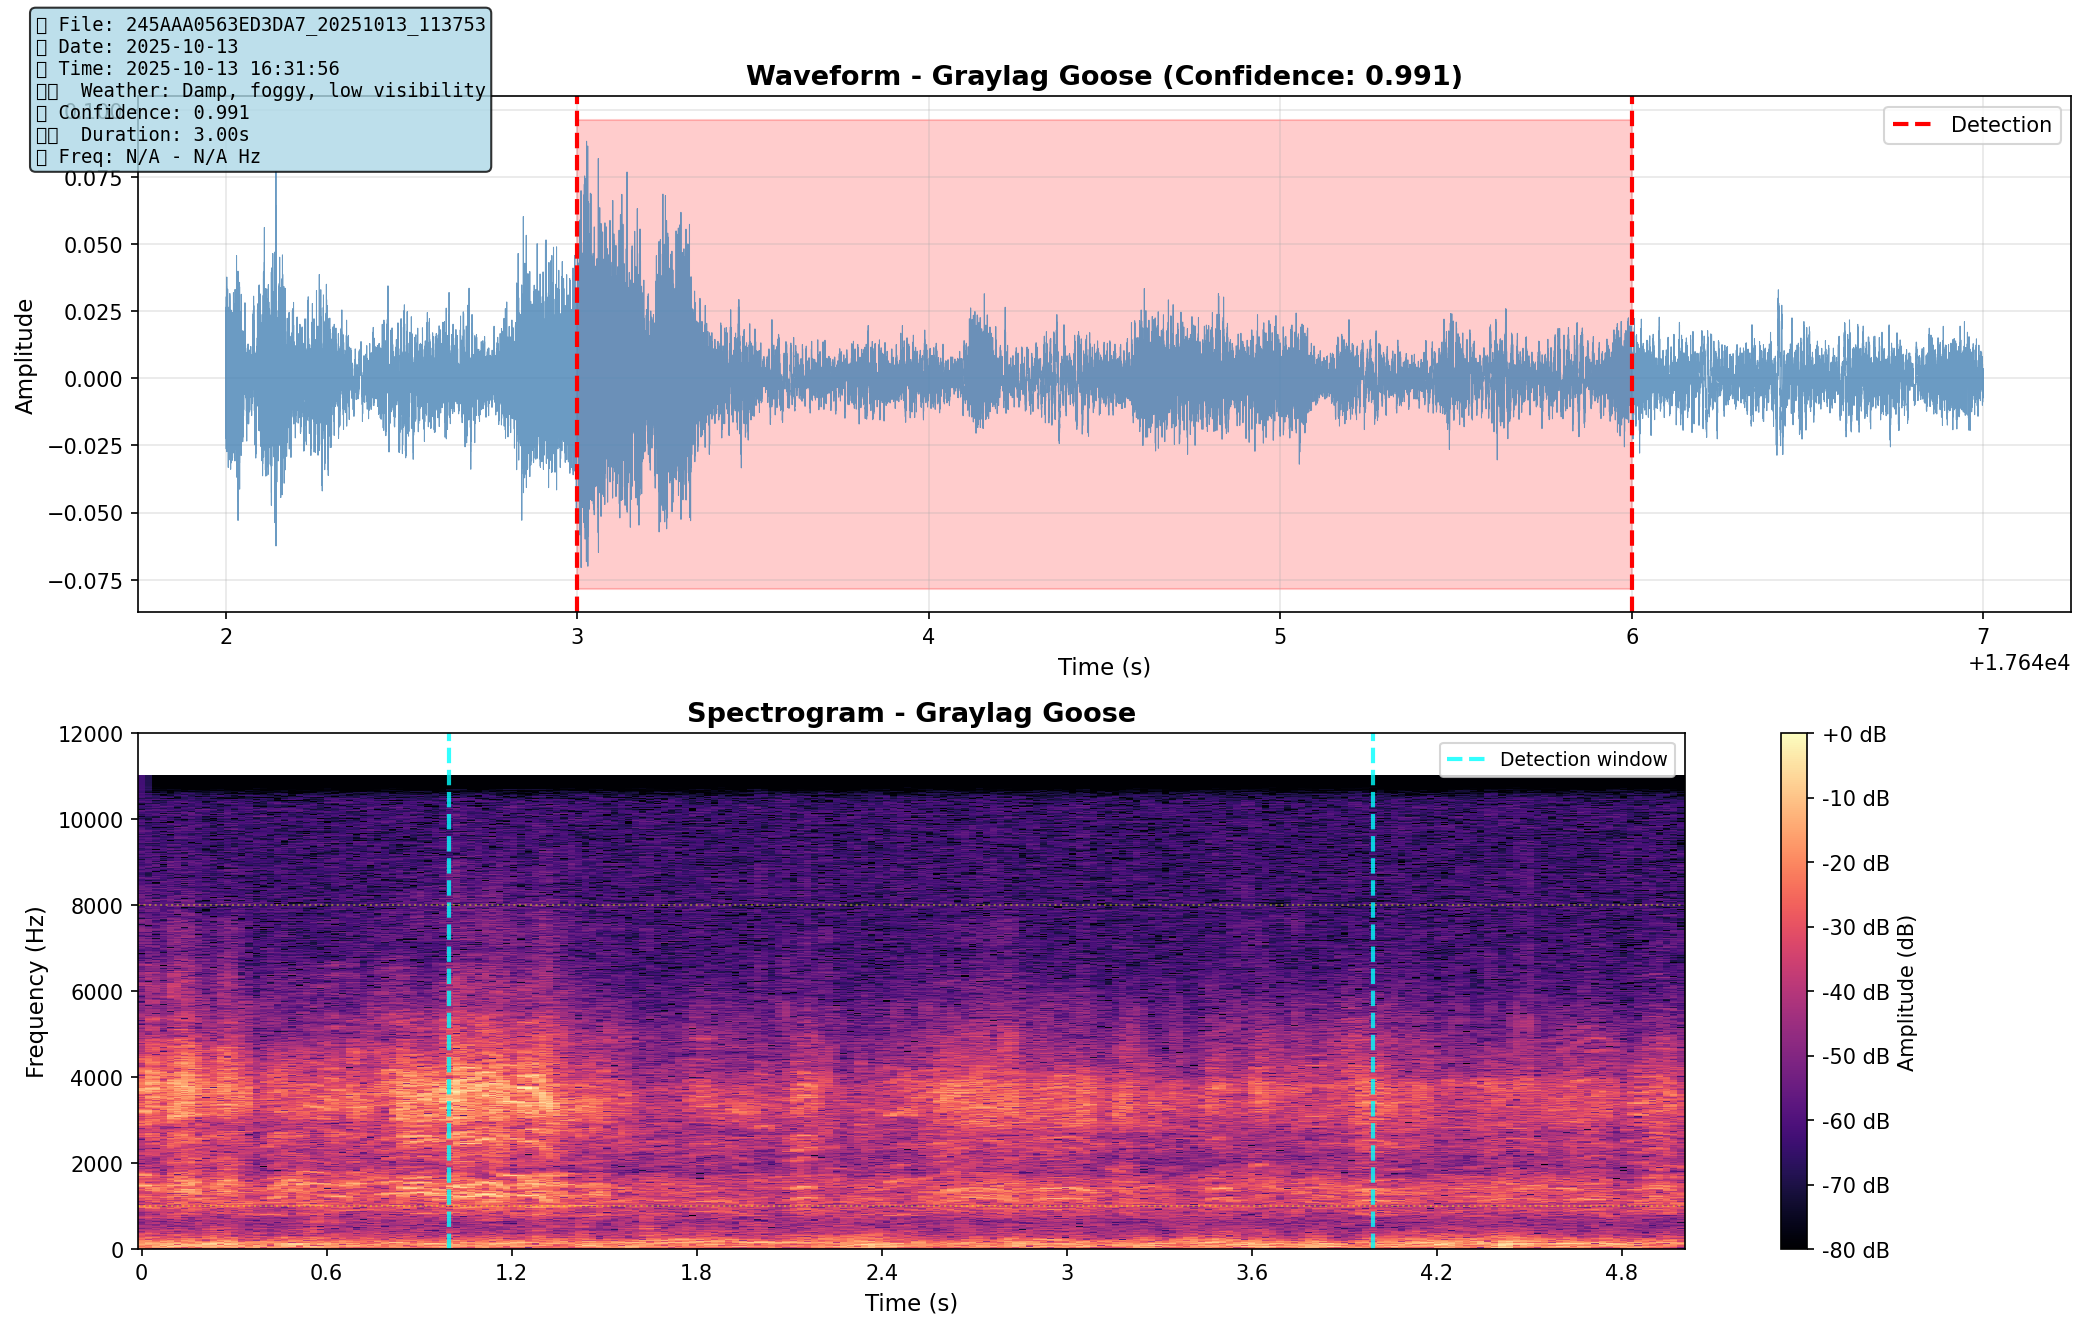
\includegraphics[width=\textwidth]{figures/spectrogram_graylag.png}
\caption{Graylag Goose contact call}
\end{subfigure}
\hfill
\begin{subfigure}{0.45\textwidth}
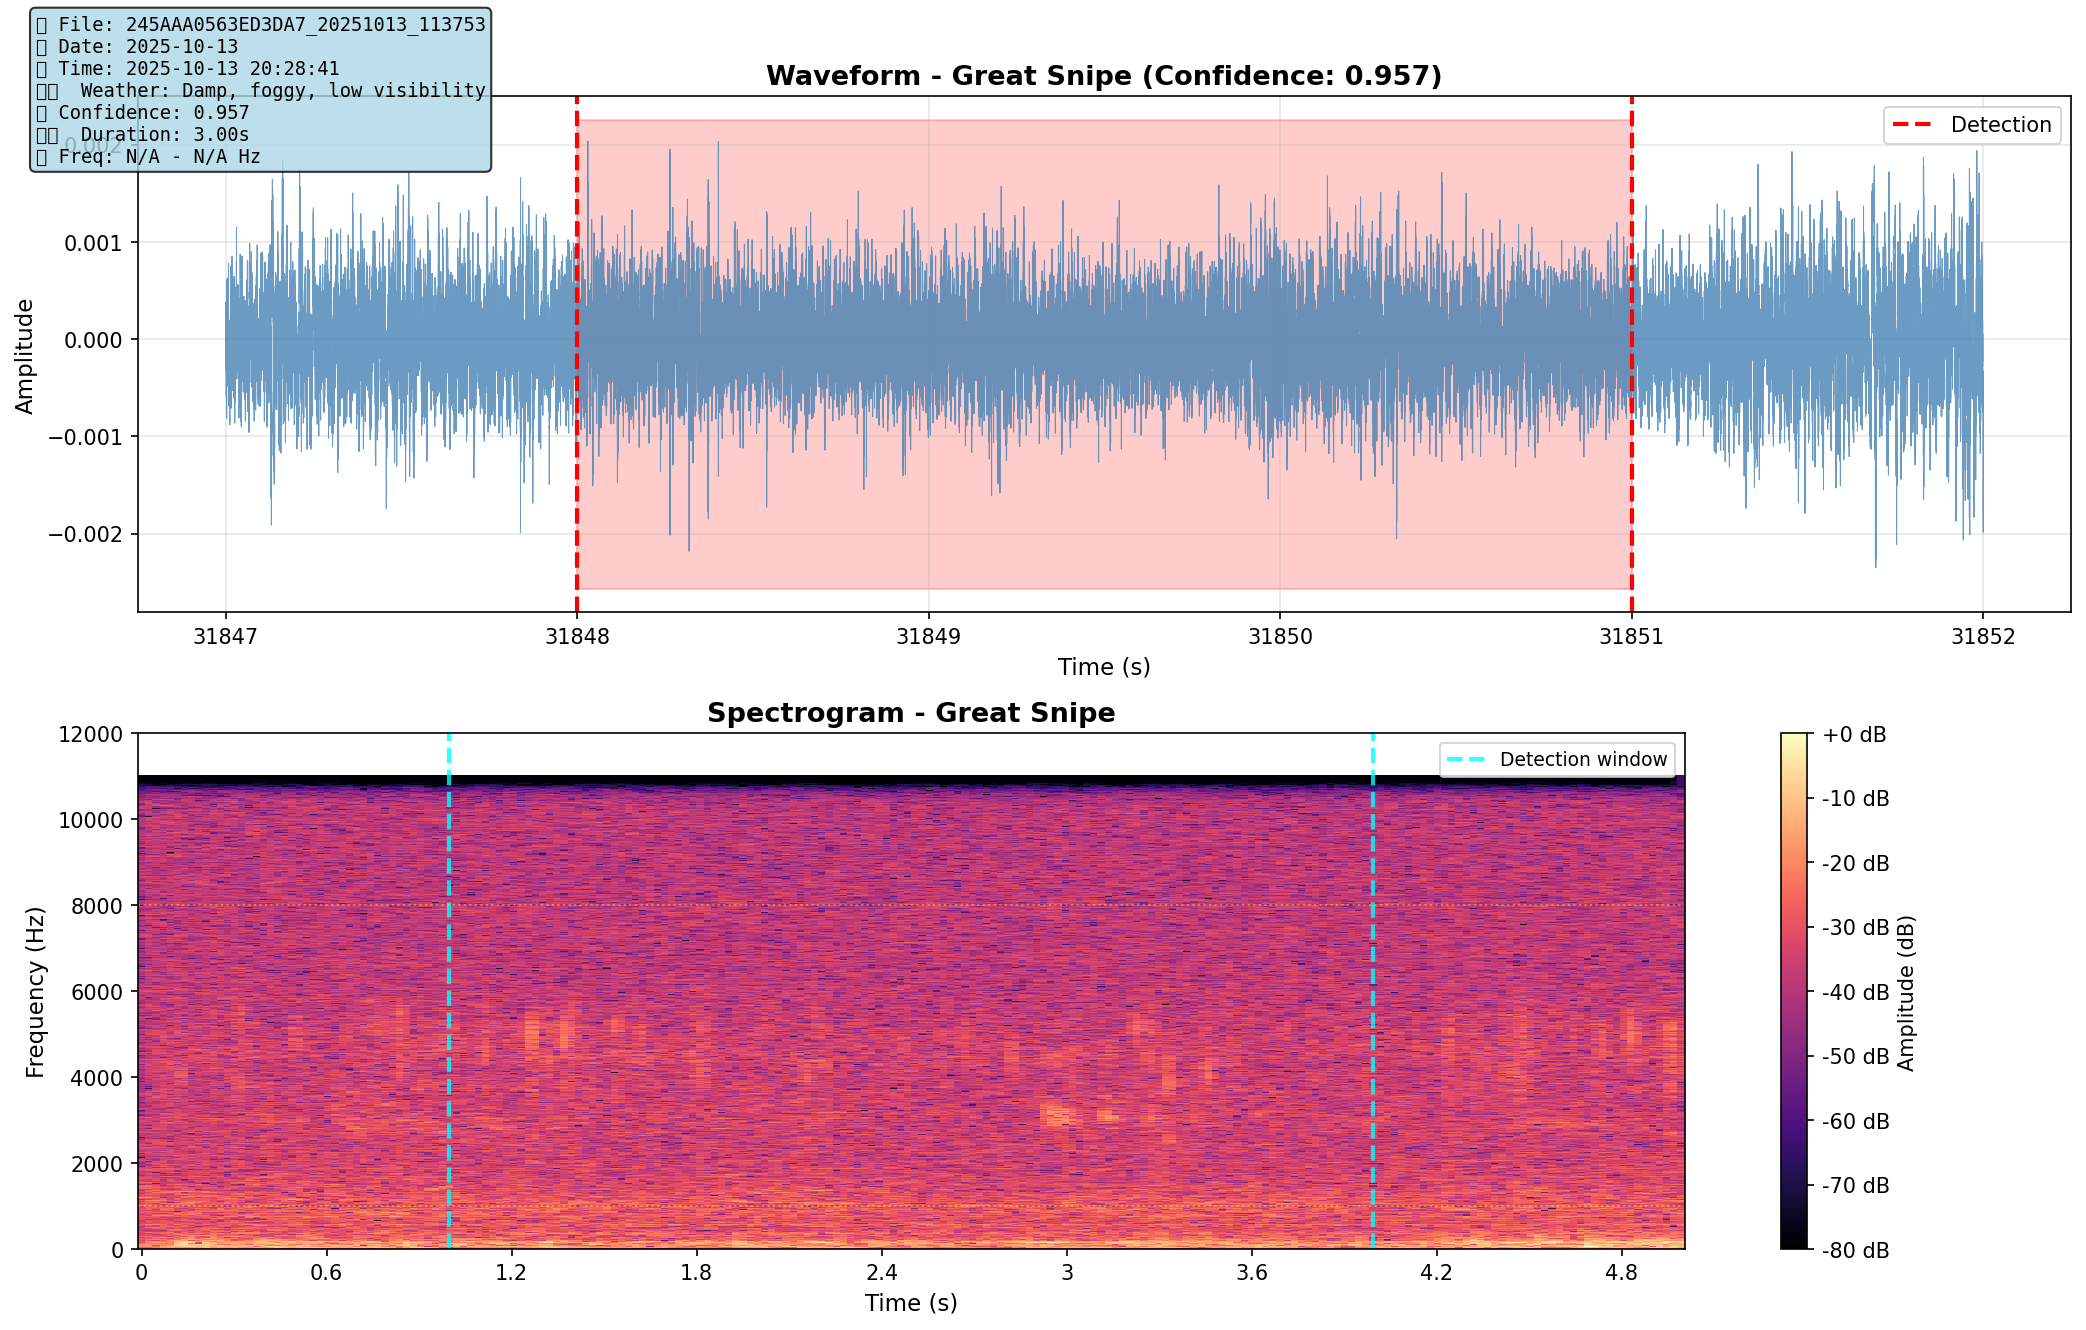
\includegraphics[width=\textwidth]{figures/spectrogram_snipe.png}
\caption{Great Snipe lek display}
\end{subfigure}

\begin{subfigure}{0.45\textwidth}
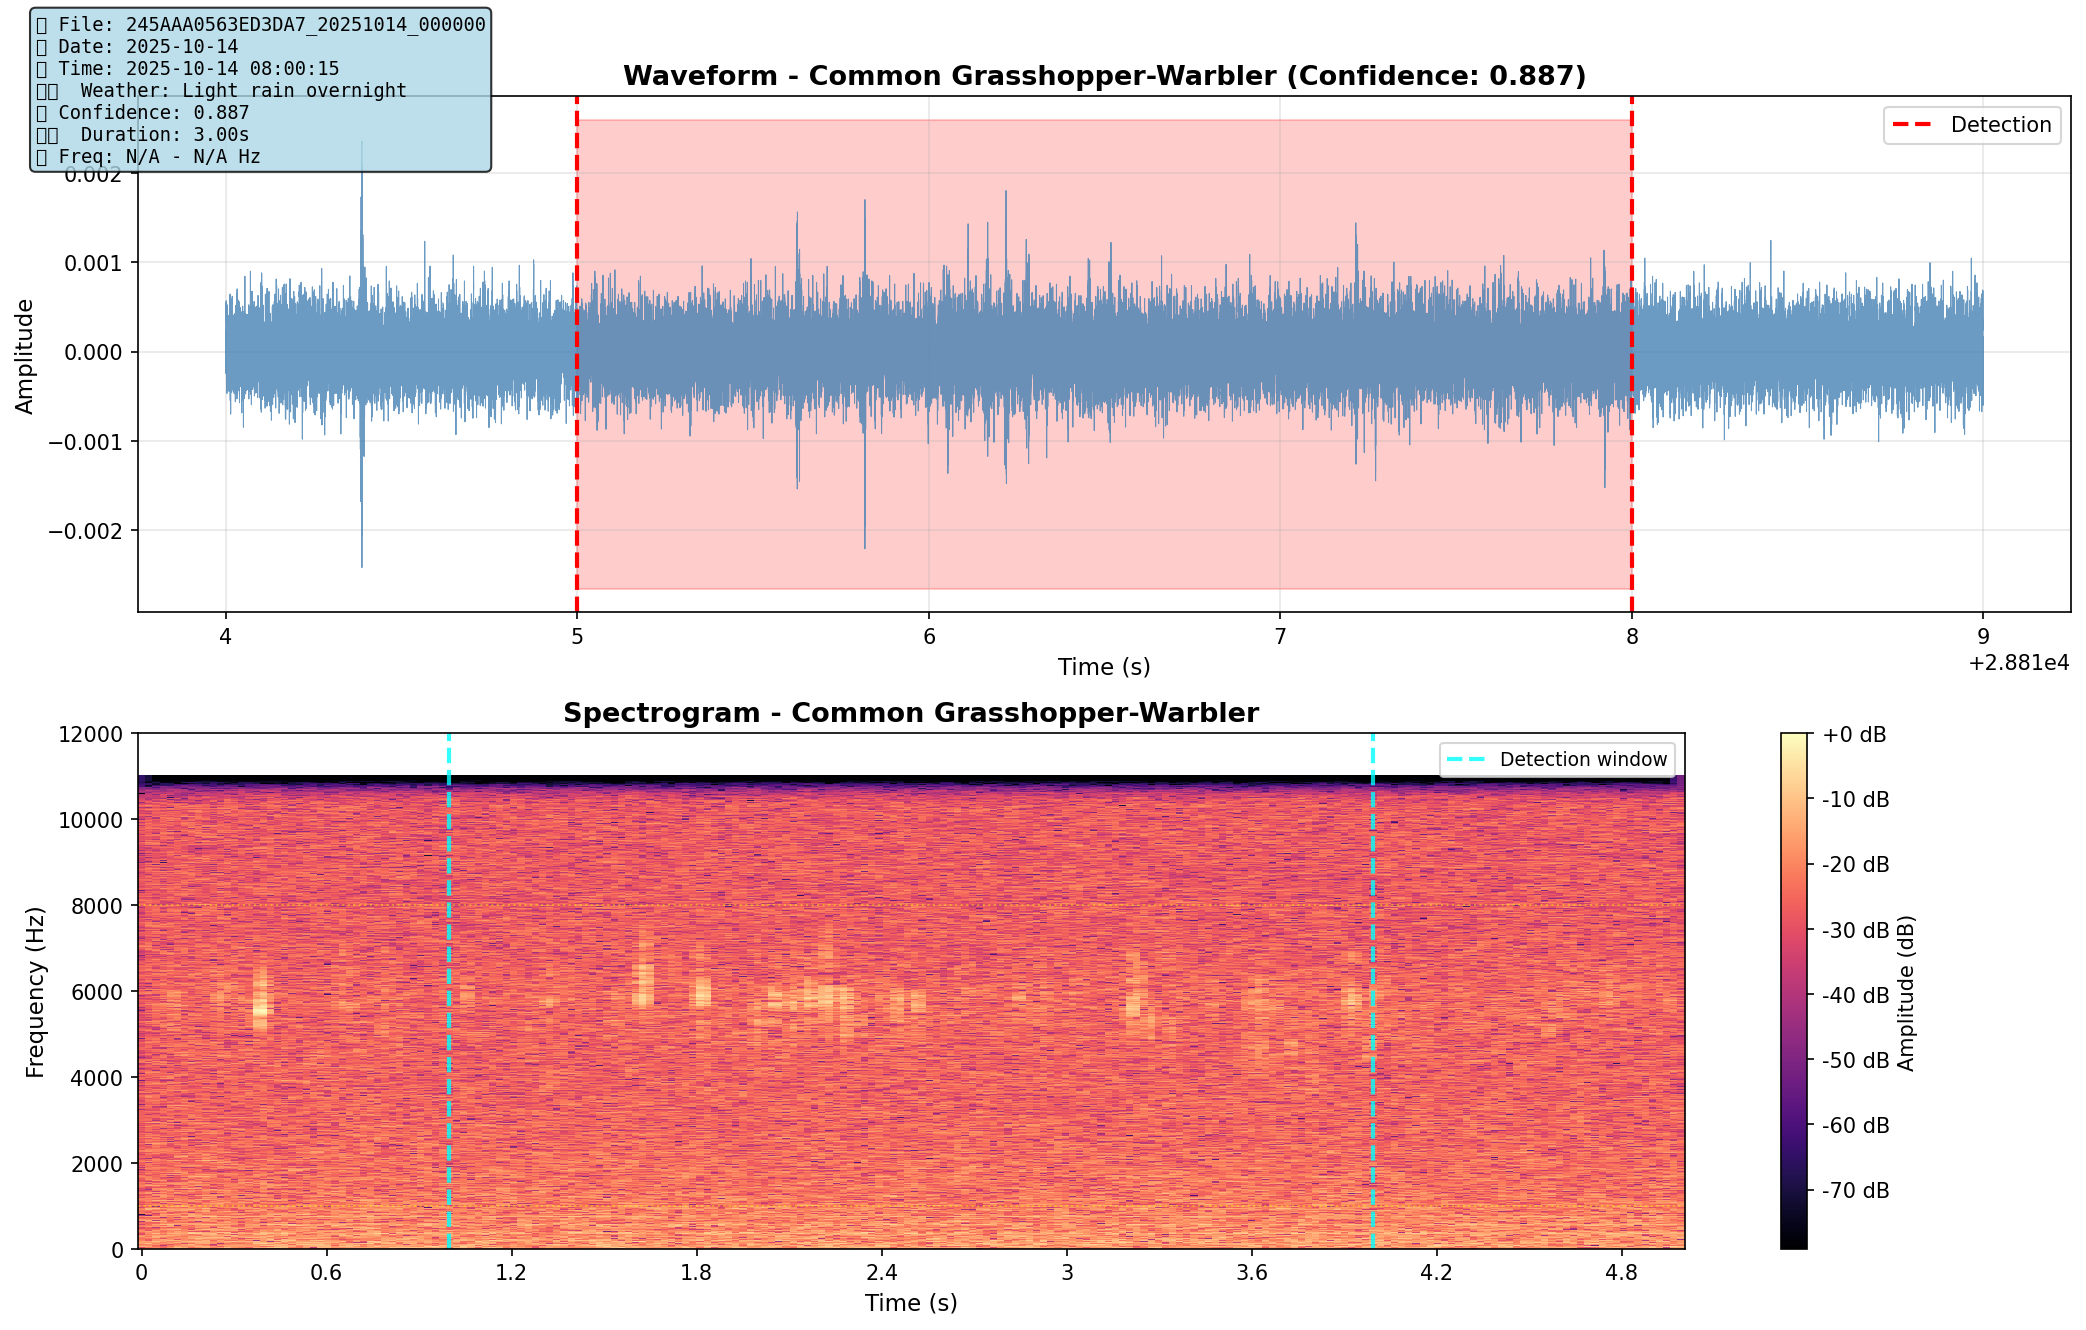
\includegraphics[width=\textwidth]{figures/spectrogram_grasshopper.png}
\caption{Common Grasshopper-Warbler trill}
\end{subfigure}
\hfill
\begin{subfigure}{0.45\textwidth}
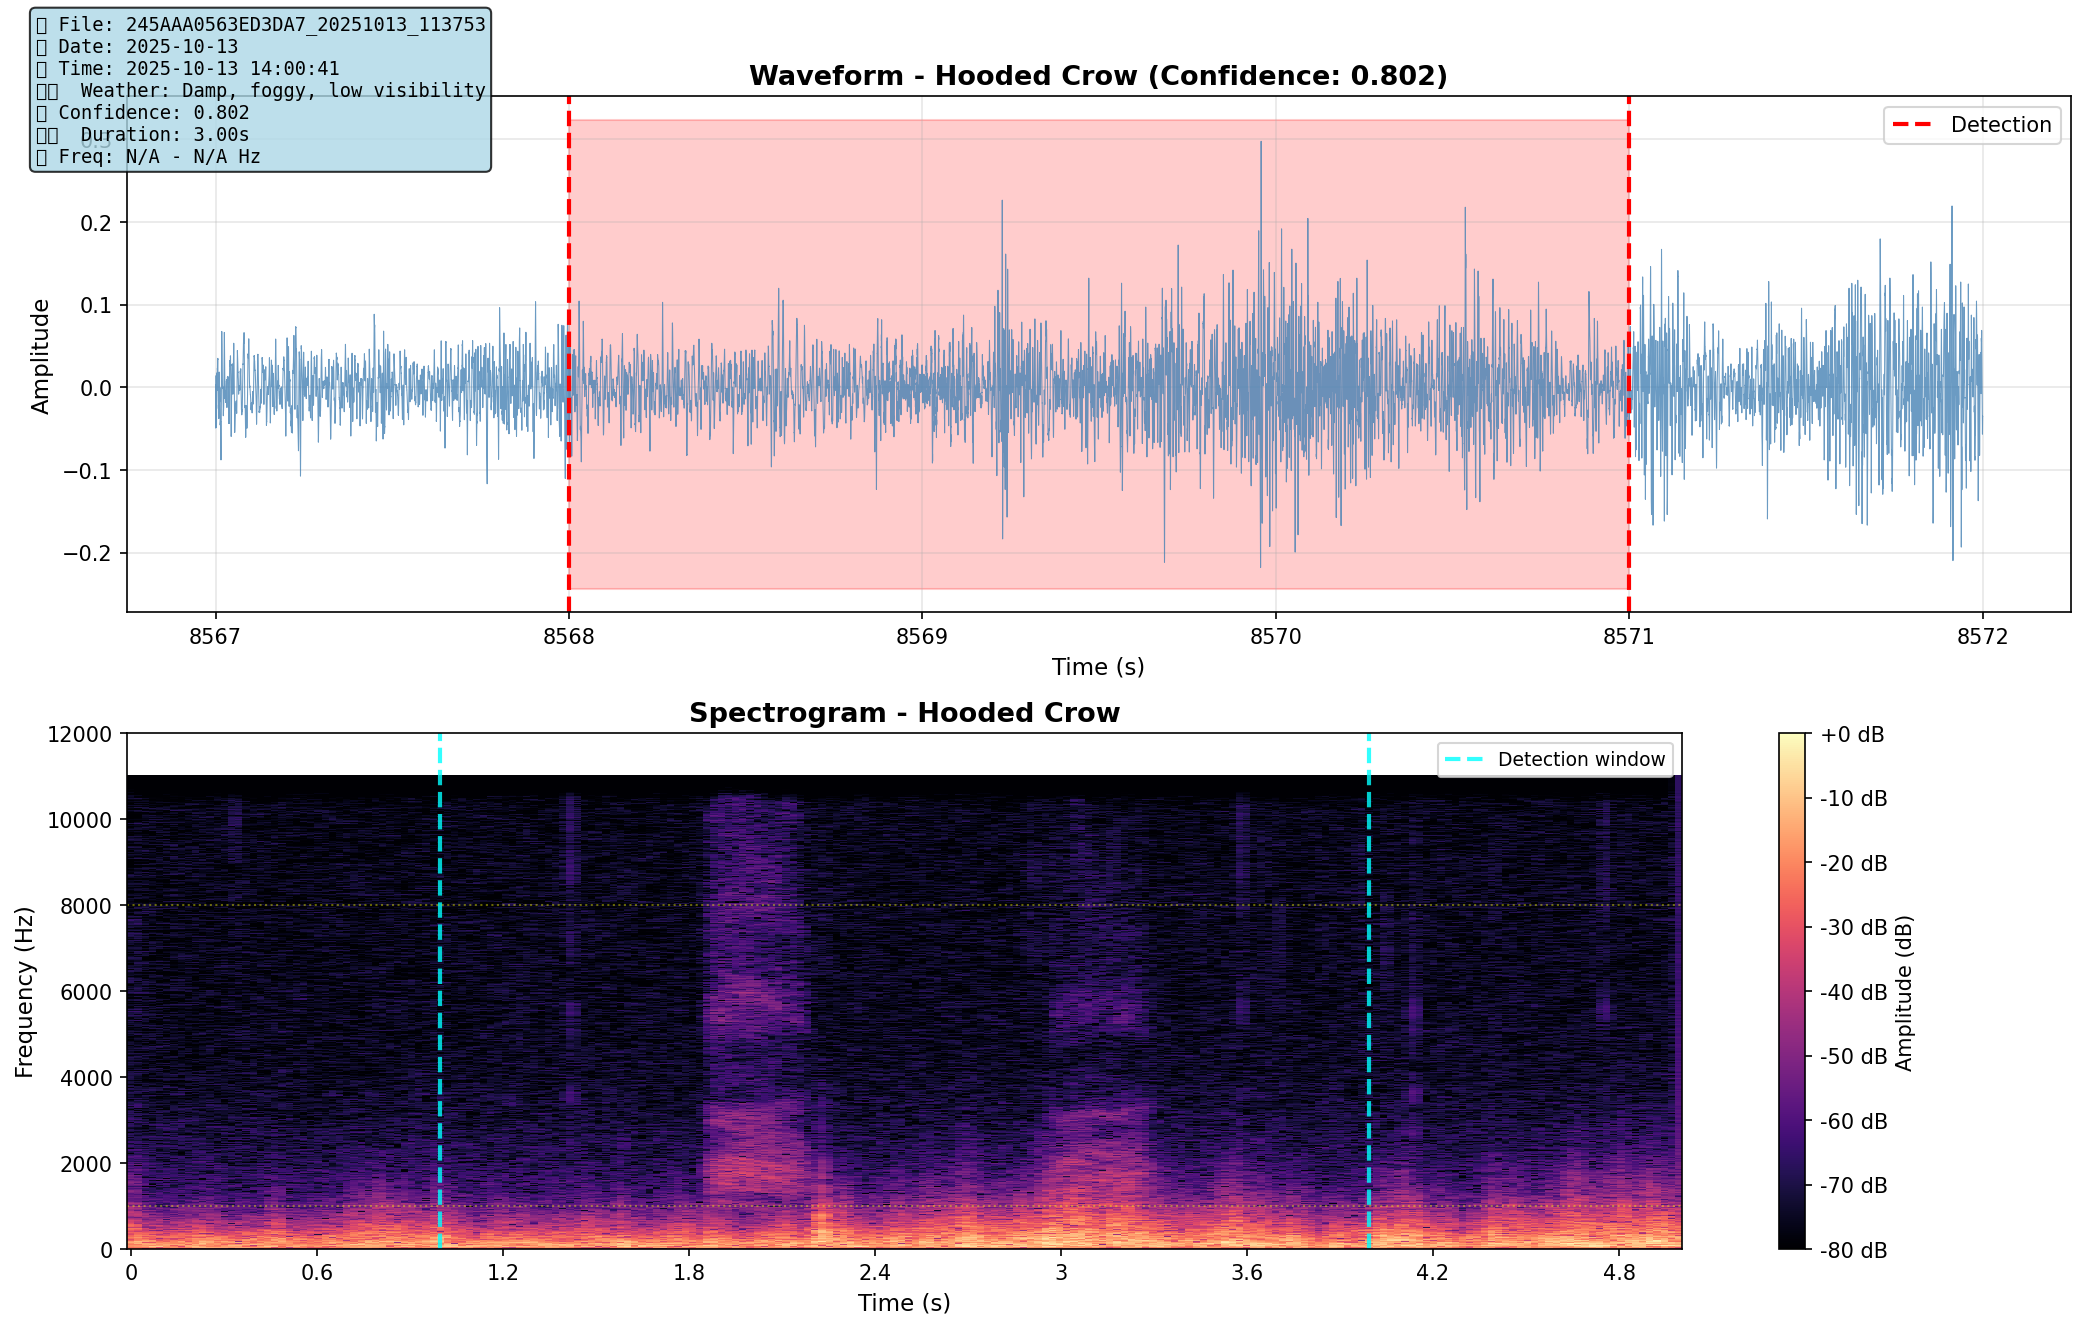
\includegraphics[width=\textwidth]{figures/spectrogram_crow.png}
\caption{Hooded Crow alarm call}
\end{subfigure}

\caption{Representative spectrograms for four key species. All spectrograms: 2048-point FFT, 512-point hop length, Hann window, 0--12 kHz range. Time scale: 0--5 seconds.}
\label{fig:spectrograms}
\end{figure}

\subsection{Weather Data}

Table \ref{tab:weather} summarizes meteorological conditions during recording period.

\begin{table}[H]
\centering
\caption{Weather conditions summary}
\label{tab:weather}
\begin{tabular}{llr}
\toprule
\textbf{Parameter} & \textbf{Value} & \textbf{Coverage} \\
\midrule
Temperature range & 7--11°C & 100\% \\
Precipitation & Rain & 80\% \\
Fog/mist & Dense & 60\% \\
Wind speed & Light--moderate & 100\% \\
Cloud cover & Overcast & 95\% \\
\bottomrule
\end{tabular}
\end{table}

\subsection{Data Access}

All supplementary data available at:

\begin{itemize}
\item \textbf{Interactive website:} \url{https://ziforge.github.io/gaulosen-study/}
\item \textbf{GitHub repository:} \url{https://github.com/Ziforge/gaulosen-study}
\item \textbf{Species gallery:} 82 species with spectrograms and audio samples
\item \textbf{Behavioral analysis datasets:} Flock events, co-occurrences, temporal patterns
\item \textbf{Analysis code:} Python scripts for BirdNET processing, audio enhancement, and visualization
\end{itemize}

\end{document}
